% Chapter Template

\chapter{Ensayos y resultados} % Main chapter title
En esta seccion se presentan los resultados obtenidos del desarrollo de hardware y software. Se analiza el cumplimiento de requisitos de desempeno impuestos por el cliente y finalmente, se exponen resultados de un ensayo \textit{end-to-end} con la red LoRaWAN.\\
\label{Chapter4} % Change X to a consecutive number; for referencing this chapter elsewhere, use \ref{ChapterX}
%----------------------------------------------------------------------------------------
%	SECTION 1
%----------------------------------------------------------------------------------------
\section{Circuito impreso desarrollado}
\label{sec:pruebasHW}
Gracias al desarrollo temprano de la primera placa prototipo de la figura \ref{fig:placaprototipo}, se realizaron las primeras validaciones de diseño de circuitos y selección de componentes para las diferentes etapas del hardware presentadas en \ref{seccion_hardware}.\\
Disponer de una placa con la mayoría de las etapas ya montadas, soldadas y depuradas, ayudó a reducir fallas eléctricas tales como falsos contactos que ocurrieron al usar protoboards.\\
% TODO: \usepackage{graphicx} required
\begin{figure}[h]
	\centering
	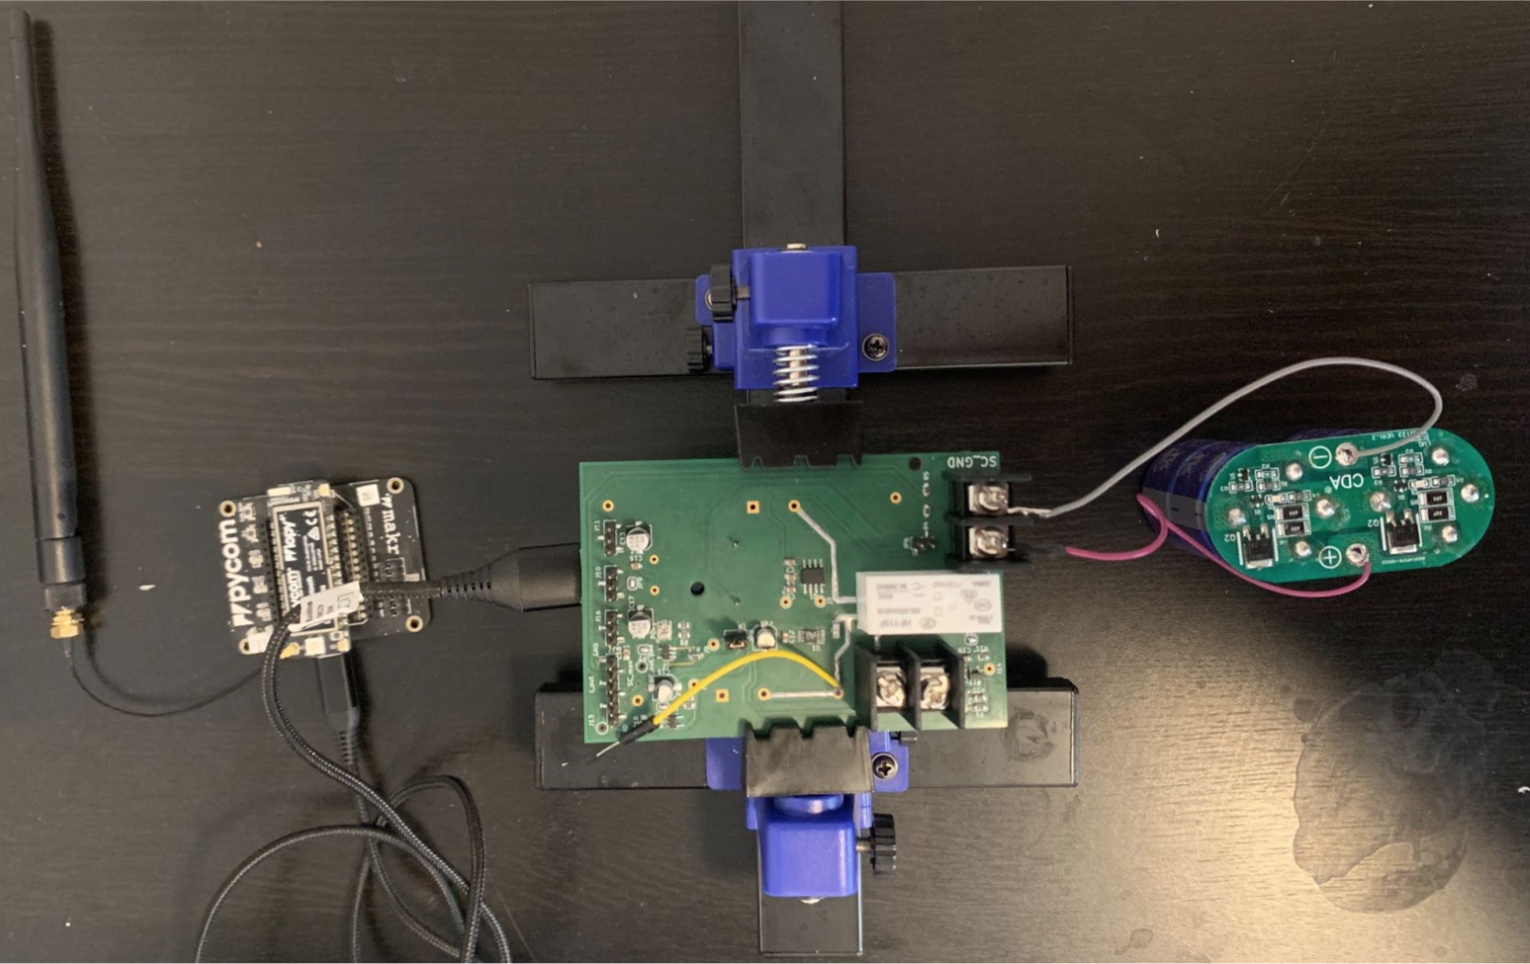
\includegraphics[width=0.9\linewidth]{Figures/placa_prototipo}
	\caption{Placa prototipo desarrollada para validacion de diseno de etapas.}
	\label{fig:placaprototipo}
\end{figure}\\
Una vez validados los diseños mediante la primera placa, se desarrolló la placa final presentada en las figuras \ref{fig:pcbfinaltop} y \ref{fig:pcbfinabottom}. Esta, a diferencia de la primera versi\'{o}n integra toda las etapas en un único circuito impreso.\\
% TODO: \usepackage{graphicx} required
\begin{figure}[h!]
	\centering
	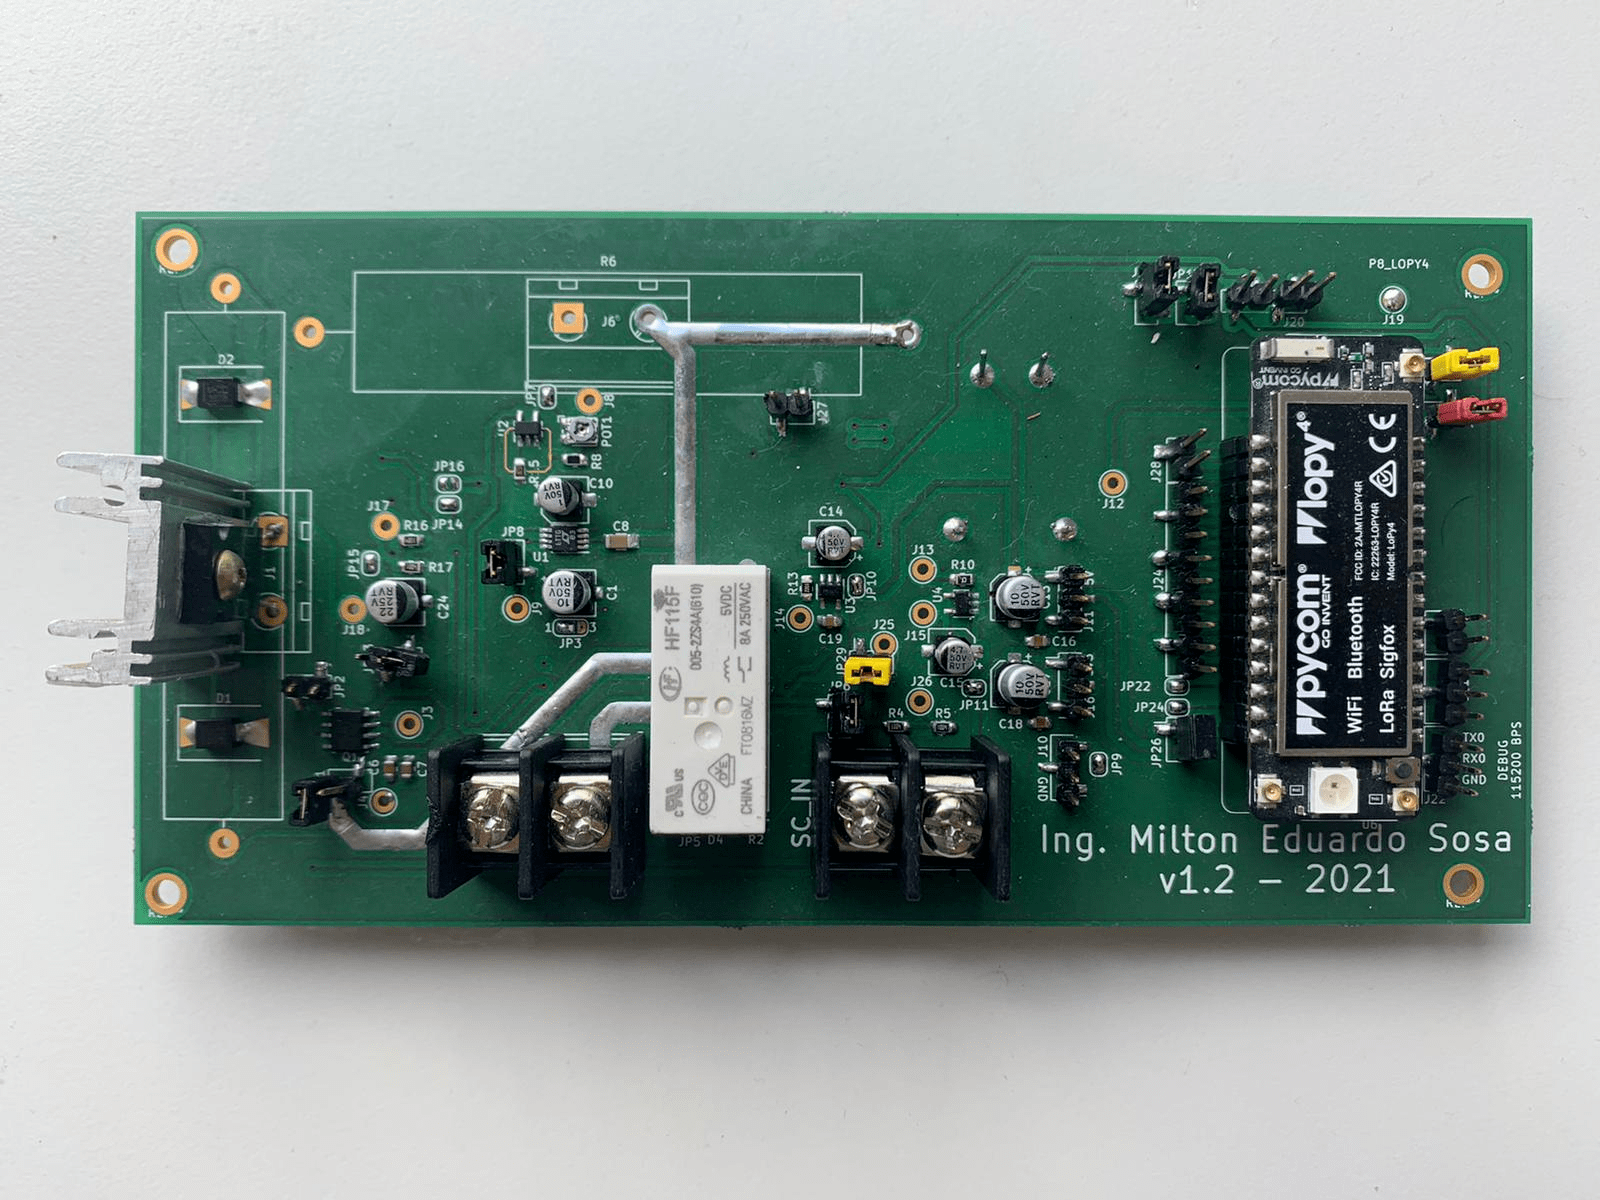
\includegraphics[width=0.8\linewidth]{Figures/pcb_final_TOP}
	\caption{Lado TOP del circuito impreso final integrando todas las etapas.}
	\label{fig:pcbfinaltop}
\end{figure}\\
% TODO: \usepackage{graphicx} required
\begin{figure}[h!]
	\centering
	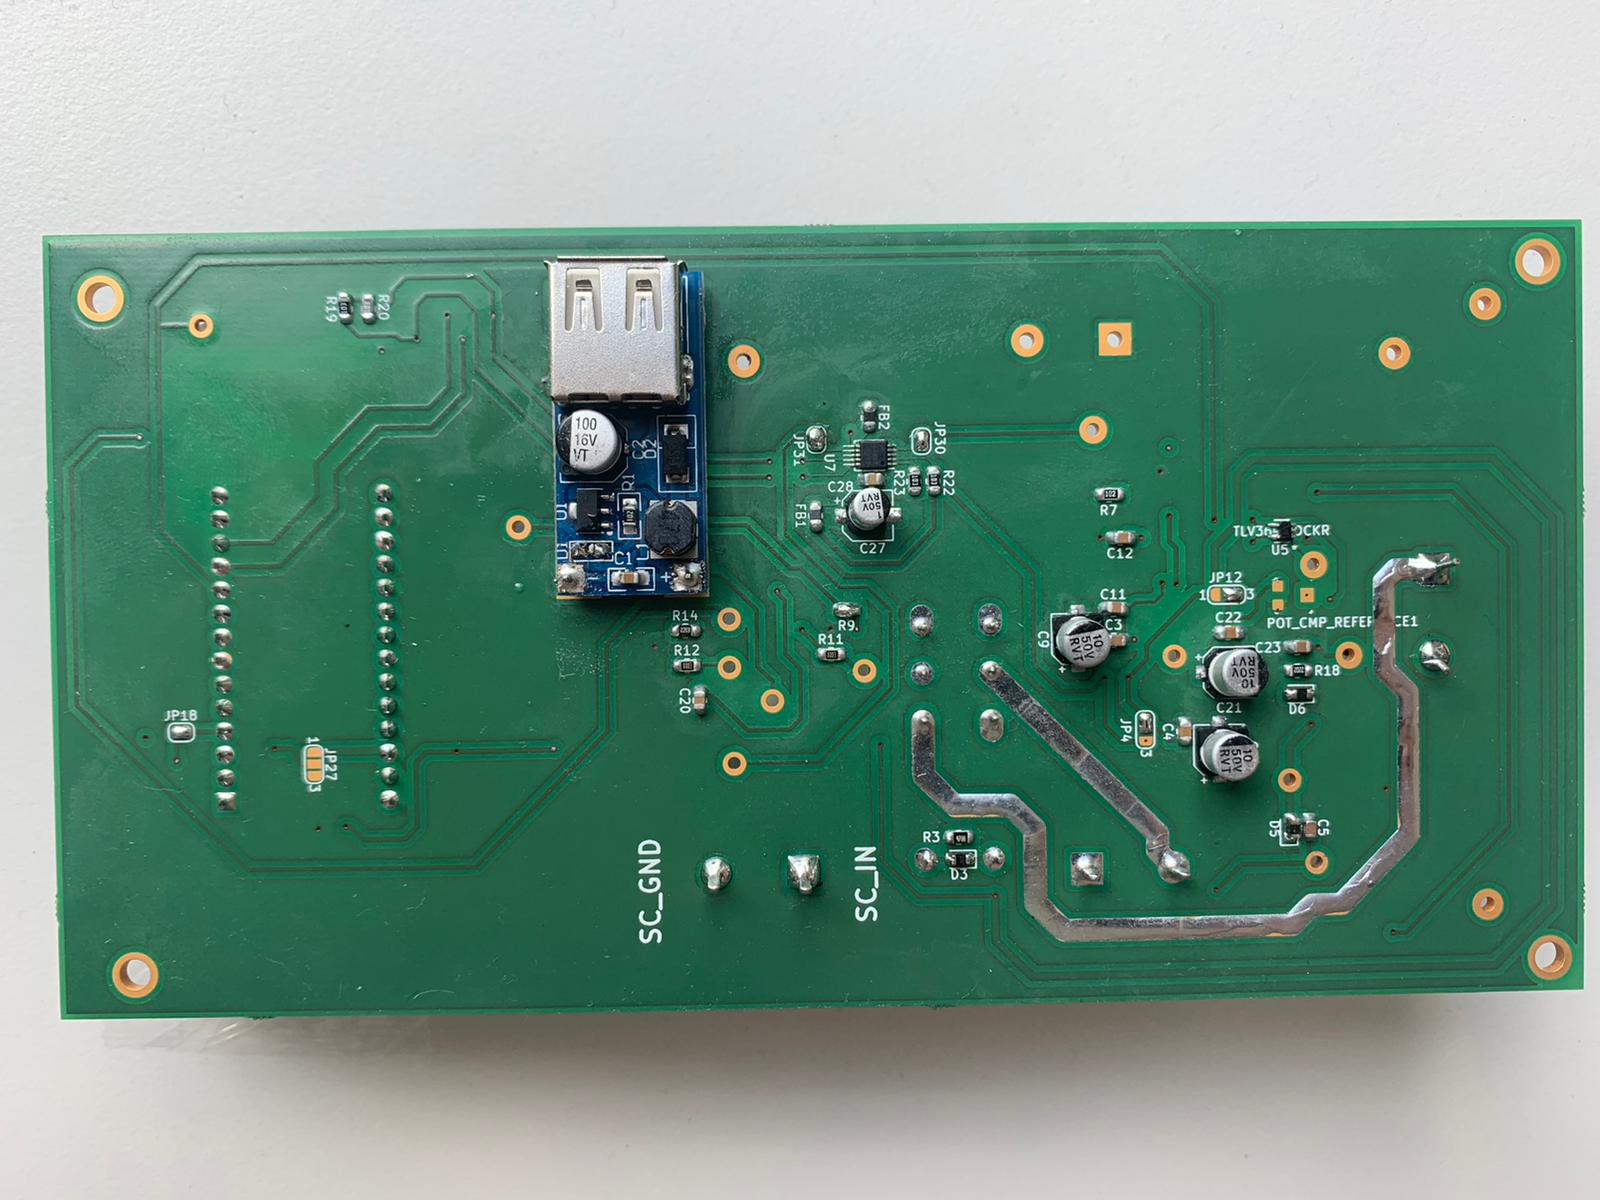
\includegraphics[width=0.8\linewidth]{Figures/pcb_fina_bottom}
	\caption{Lado BOTTOM del circuito impreso final que alberga todas las etapas.}
	\label{fig:pcbfinabottom}
\end{figure}


\section{Medidor de valor RMS}\label{ensayo_medidor_rms}


\section{Circuito detector de cortes}

\section{Consumo en deep sleep}
Debido a la imposibilidad de poder acceder a un laboratorio con instrumental de precisión, las mediciones tomadas en los ensayos se realizaron por partes y en diferentes turnos.\\
Como instrumento de medición se contó únicamente con un multímetro de la marca HoldPeak modelo HP-770d [REFERENCIA AL DATASHEET DEL MULTIMETRO] y sus caracteristicas se muestran en la tabla [TABLA MULTIMETRO].\\
El instrumento utilizado tiene un rango de medición de corriente que permite medir desde los uA hasta 400 mA. Este rango pareció suficiente para la medición de corriente en ambos estados sin la necesidad de cambiar de escala. Sin embargo, en las primeras rondas de medición se advirtió que al salir del modo ahorro de energía y transmitir, la corriente consumida por el hardware generó una tensión de burden en el instrumento que causó que el microcontrolador se reseteara por desvanecimiento (Brown Out Reset-).\\
Como solución, para el ensayo de consumo en deep sleep se grabó sobre la LoPy4 una versión de firmware que llevó al hardware al modo ahorro de energía apenas se energizo por al menos 10 minutos. Un tiempo suficiente para registrar el consumo de corriente en este modo.\\
Para la medición de consumo durante la transmisión, se programó la versión final de firmware. Para sortear el problema de reseteo por desvanecimiento se utilizó la escala de amperes en conjunto con la función que retiene el pico máximo de la señal.\\
La tabla TTT, expone los resultados promedio para un total de 10 mediciones efectuadas en cada modo.\\
% \usepackage{color}
\begin{table}[h]
	\centering
	\caption{Consumo máximo registrado en los diferentes modos.}
	\begin{tabular}{cc} 
		\hline
		Modo                                                & \begin{tabular}[c]{@{}c@{}}Consumo\\\textcolor[rgb]{0.302,0.318,0.337}{máximo}\end{tabular}  \\ 
		\hline
		\begin{tabular}[c]{@{}c@{}}Deep\\sleep\end{tabular} & 62 uA                                                                                        \\
		Transmisión                                         & 127 mA                                                                                       \\
		\hline
	\end{tabular}\label{tabla_consumos}
\end{table}\\
Si bien el perfil estimado de consumo del hardware es similar al presentado en \ref{fig:ciclodeepsleep}, por falta de equipamiento no se ha podido capturar un oscilograma para graficar su perfil exacto. Tal gráfico se podría haber adquirido con un multimetro de 7 ½ dígitos con la función de almacenamiento.\\
Desenergizar toda la electrónica salvo al microcontrolador, ha reducido el consumo total de la electrónica al orden de los microamperes. Este valor de consumo registrado, se encuentra debajo de lo requerido por el cliente en \ref{req_deep_sleep} e implica un aumento en la autonomía del acumulador.\\


\section{Autonom\'{i}a del supercapacitor}
Este ensayo tuvo como objetivo principal, verificar el cumplimiento del requerimiento \ref{req_autonomia}.\\
El ensayo comenzo con el banco de supercapacitores completamente cargado y 

\section{Ensayo end-to-end}